\documentclass[tikz,border=8pt]{standalone}
\usepackage{tikz}
\usepackage{amsmath}
\usepackage{amssymb}
\usetikzlibrary{positioning, arrows.meta, fit, calc, backgrounds}

%% ── colour palette ──────────────────────────────────────────────────────────
\definecolor{corecol}{RGB}{41,98,178}
\definecolor{corelite}{RGB}{210,225,255}
\definecolor{arcol}{RGB}{200,80,20}
\definecolor{disccol}{RGB}{120,40,170}
\definecolor{elfcol}{RGB}{15,130,90}
\definecolor{frozcol}{RGB}{150,35,35}
\definecolor{optcol}{RGB}{90,90,90}

\begin{document}
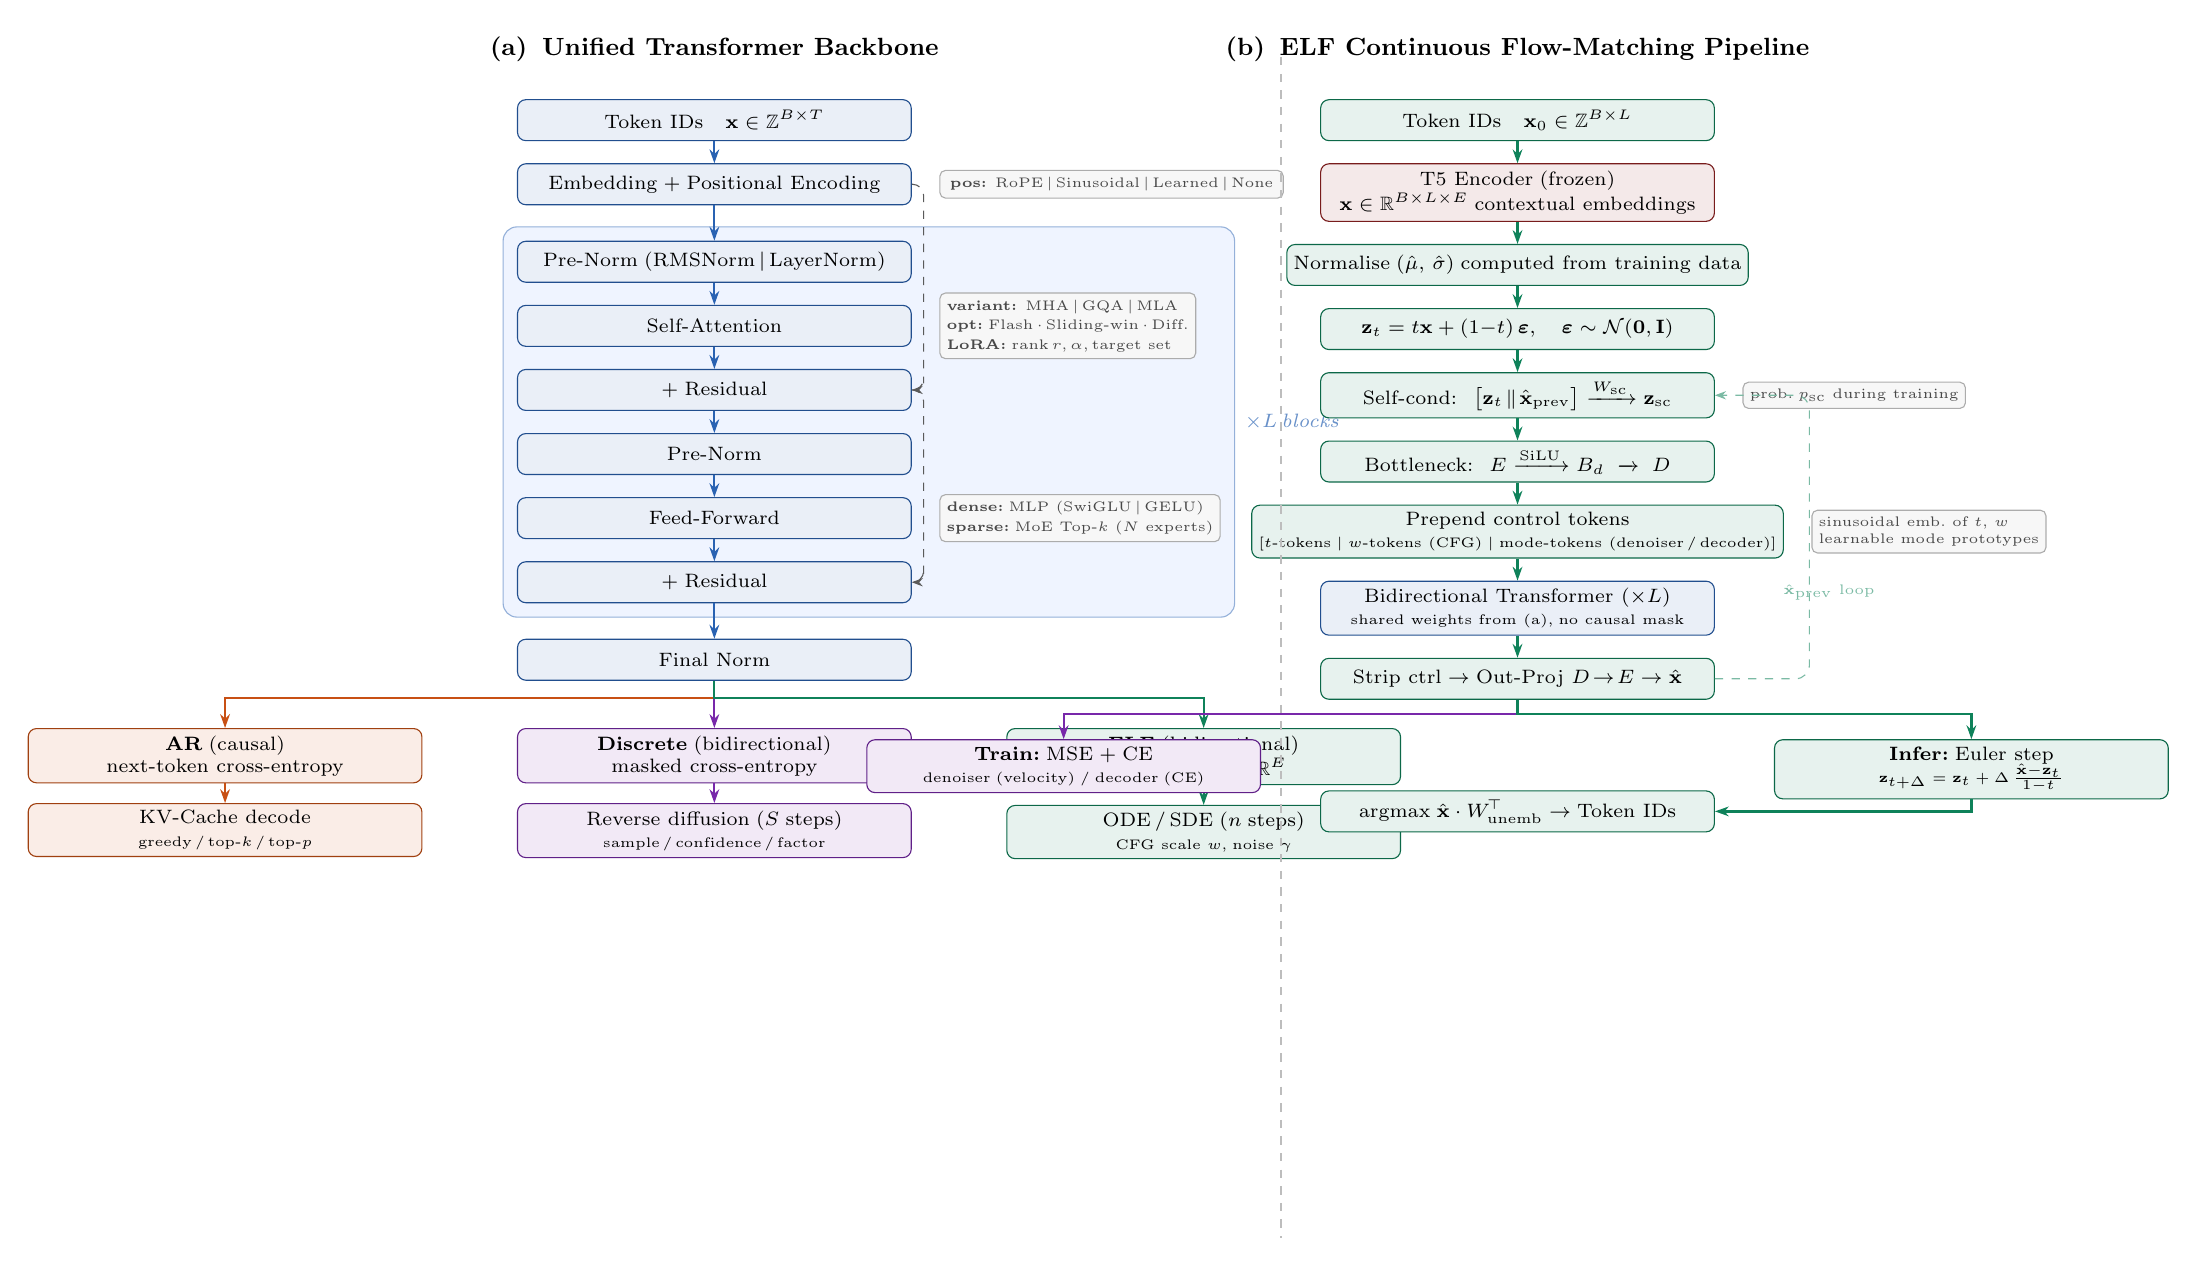
\begin{tikzpicture}[
  node distance = 0.28cm and 0.3cm,
  every node/.style = {font=\scriptsize},
  %% main block style (colour argument)
  mb/.style = {draw=#1!80!black, fill=#1!10, rounded corners=3pt,
               minimum width=5.0cm, minimum height=0.52cm,
               align=center, inner sep=2.5pt},
  mb/.default = corecol,
  %% option / annotation box
  ob/.style = {draw=optcol!50, fill=optcol!5, rounded corners=2pt,
               font=\tiny, align=left, inner sep=2.5pt, text=optcol!80!black},
  %% coloured arrow (default = core blue)
  arr/.style = {-{Stealth[length=5pt,width=3.5pt]}, thick, color=#1},
  arr/.default = corecol,
  %% dashed residual skip
  sk/.style = {-{Stealth[length=4pt]}, dashed, optcol, rounded corners=4pt},
]

%%============================================================
%%  PANEL (a) — Unified Transformer Backbone
%%============================================================

\node[mb] (A0) {Token IDs\quad$\mathbf{x}\in\mathbb{Z}^{B\times T}$};

\node[mb, below=of A0] (A1) {Embedding\;+\;Positional Encoding};
\node[ob, right=0.35cm of A1] (A1o)
  {\,\textbf{pos:} RoPE\,$|$\,Sinusoidal\,$|$\,Learned\,$|$\,None\,};

%%── block internals ──────────────────────────────────────────
\node[mb, below=0.45cm of A1] (A2) {Pre-Norm\;(RMSNorm\,$|$\,LayerNorm)};

\node[mb, below=of A2] (A3) {Self-Attention};
\node[ob, right=0.35cm of A3] (A3o)
  {\textbf{variant:} MHA\,$|$\,GQA\,$|$\,MLA\\[1pt]
   \textbf{opt:}\;Flash\,$\cdot$\,Sliding-win\,$\cdot$\,Diff.\\[1pt]
   \textbf{LoRA:}\;rank\,$r$,\,$\alpha$,\,target set};

\node[mb, below=of A3] (A4) {$+\;$Residual};

\node[mb, below=of A4] (A5) {Pre-Norm};

\node[mb, below=of A5] (A6) {Feed-Forward};
\node[ob, right=0.35cm of A6] (A6o)
  {\textbf{dense:}\;MLP (SwiGLU\,$|$\,GELU)\\[1pt]
   \textbf{sparse:}\;MoE Top-$k$ ($N$ experts)};

\node[mb, below=of A6] (A7) {$+\;$Residual};

%% block frame (drawn on background layer after all nodes are placed)
\begin{pgfonlayer}{background}
  \node[draw=corecol!50, fill=corelite!35, rounded corners=5pt,
        fit=(A2)(A7)(A3o)(A6o), inner sep=5pt,
        label={[font=\scriptsize\itshape, text=corecol!70]right:$\times L$\,blocks}]
       (Aframe) {};
\end{pgfonlayer}
%%─────────────────────────────────────────────────────────────

\node[mb, below=0.45cm of A7] (A8) {Final Norm};

%% paradigm heads
\node[mb=arcol,   below left =0.60cm and 1.20cm of A8] (Aar)
  {\textbf{AR}\;(causal)\\\scriptsize next-token cross-entropy};
\node[mb=disccol, below=0.60cm of A8] (Adisc)
  {\textbf{Discrete}\;(bidirectional)\\\scriptsize masked cross-entropy};
\node[mb=elfcol,  below right=0.60cm and 1.20cm of A8] (Aelf)
  {\textbf{ELF}\;(bidirectional)\\\scriptsize MSE\,+\,CE in $\mathbb{R}^E$};

\node[mb=arcol,   below=0.25cm of Aar]   (Aar2)
  {KV-Cache decode\\\tiny greedy\,/\,top-$k$\,/\,top-$p$};
\node[mb=disccol, below=0.25cm of Adisc] (Adisc2)
  {Reverse diffusion\;($S$\;steps)\\\tiny sample\,/\,confidence\,/\,factor};
\node[mb=elfcol,  below=0.25cm of Aelf]  (Aelf2)
  {ODE\,/\,SDE\;($n$\;steps)\\\tiny CFG scale $w$,\;noise $\gamma$};

%%── arrows ───────────────────────────────────────────────────
\draw[arr] (A0) -- (A1);
\draw[arr] (A1) -- (A2);
\draw[arr] (A2) -- (A3);
\draw[arr] (A3) -- (A4);
\draw[arr] (A4) -- (A5);
\draw[arr] (A5) -- (A6);
\draw[arr] (A6) -- (A7);
\draw[arr] (A7) -- (A8);

\draw[arr=arcol]   (A8.south) -- ++(0,-.22) -| (Aar.north);
\draw[arr=disccol] (A8)       -- (Adisc);
\draw[arr=elfcol]  (A8.south) -- ++(0,-.22) -| (Aelf.north);

\draw[arr=arcol]   (Aar)   -- (Aar2);
\draw[arr=disccol] (Adisc) -- (Adisc2);
\draw[arr=elfcol]  (Aelf)  -- (Aelf2);

%% residual skip connections
\draw[sk] (A1.east) -- ++(0.15,0)
          |- ($(A4.east)+(0.15,0)$) -- (A4.east);
\draw[sk] (A4.east) -- ++(0.15,0)
          |- ($(A7.east)+(0.15,0)$) -- (A7.east);

\node[font=\small\bfseries, above=0.35cm of A0]
  {\textbf{(a)}\enspace Unified Transformer Backbone};

%%============================================================
%%  PANEL (b) — ELF Continuous Flow-Matching Pipeline
%%============================================================
\begin{scope}[xshift=10.2cm]

\node[mb=elfcol] (B0)
  {Token IDs\quad$\mathbf{x}_0\in\mathbb{Z}^{B\times L}$};

\node[mb=frozcol, below=of B0] (B1)
  {T5 Encoder\;(frozen)\\\scriptsize$\mathbf{x}\in\mathbb{R}^{B\times L\times E}$\;contextual embeddings};

\node[mb=elfcol, below=of B1] (B2)
  {Normalise\;$(\hat{\mu},\,\hat{\sigma})$\;computed from training data};

\node[mb=elfcol, below=of B2] (B3)
  {$\mathbf{z}_t = t\mathbf{x}+(1{-}t)\,\boldsymbol{\varepsilon},
    \quad\boldsymbol{\varepsilon}\sim\mathcal{N}(\mathbf{0},\mathbf{I})$};

\node[mb=elfcol, below=of B3] (B4)
  {Self-cond:\;
   $\bigl[\mathbf{z}_t\!\parallel\!\hat{\mathbf{x}}_{\mathrm{prev}}\bigr]
   \xrightarrow{W_{\mathrm{sc}}}\mathbf{z}_{\mathrm{sc}}$};
\node[ob, right=0.35cm of B4] (B4o)
  {prob.\;$p_\mathrm{sc}$ during training};

\node[mb=elfcol, below=of B4] (B5)
  {Bottleneck:\;
   $E\xrightarrow{\mathrm{SiLU}}B_d\;\xrightarrow{\phantom{.}}\;D$};

\node[mb=elfcol, below=of B5] (B6)
  {Prepend control tokens\\
   {\tiny [$t$-tokens\;$|$\;$w$-tokens (CFG)\;$|$\;mode-tokens (denoiser\,/\,decoder)]}};
\node[ob, right=0.35cm of B6] (B6o)
  {sinusoidal emb.\ of $t$, $w$\\learnable mode prototypes};

\node[mb=corecol, below=of B6] (B7)
  {Bidirectional Transformer ($\times L$)\\
   {\tiny shared weights from (a),\;no causal mask}};

\node[mb=elfcol, below=of B7] (B8)
  {Strip ctrl\;$\to$\;Out-Proj $D\!\to\!E$\;$\to\hat{\mathbf{x}}$};

%% training / inference branches
\node[mb=disccol, below left =0.50cm and 0.75cm of B8] (B9a)
  {\textbf{Train:}\;MSE\;+\;CE\\
   \tiny denoiser\;(velocity)\;/\;decoder\;(CE)};
\node[mb=elfcol,  below right=0.50cm and 0.75cm of B8] (B9b)
  {\textbf{Infer:}\;Euler step\\
   \tiny$\mathbf{z}_{t+\Delta}=\mathbf{z}_t
         +\Delta\,\tfrac{\hat{\mathbf{x}}-\mathbf{z}_t}{1-t}$};

\node[mb=elfcol, below=1.15cm of B8] (B10)
  {argmax\;$\hat{\mathbf{x}}\cdot W_{\mathrm{unemb}}^{\!\top}$\;$\to$\;Token IDs};

%%── arrows (b) ───────────────────────────────────────────────
\foreach \s/\t in {B0/B1, B1/B2, B2/B3, B3/B4, B4/B5, B5/B6, B6/B7, B7/B8}
  \draw[arr=elfcol] (\s) -- (\t);

\draw[arr=disccol] (B8.south) -- ++(0,-.18) -| (B9a.north);
\draw[arr=elfcol]  (B8.south) -- ++(0,-.18) -| (B9b.north);
\draw[arr=elfcol]  (B9b.south) |- (B10.east);

%% self-conditioning feedback loop
\draw[-{Stealth[length=4pt]}, dashed, elfcol!55, rounded corners=5pt]
  (B8.east) -- ++(1.2,0) |- (B4.east);
\node[font=\tiny, elfcol!55]
  at ($(B8.east)+(1.45,0)+(0,1.10)$)
  {$\hat{\mathbf{x}}_{\mathrm{prev}}$ loop};

\node[font=\small\bfseries, above=0.35cm of B0]
  {\textbf{(b)}\enspace ELF Continuous Flow-Matching Pipeline};

\end{scope}

%%── vertical separator between the two panels ───────────────
\draw[dashed, optcol!40, thick] (7.2, 0.8) -- (7.2, -14.2);

\end{tikzpicture}
\end{document}
